\section{Fibracje kartezjańskie i kokartezjańskie}\label{cat:sec:cartesian-fibrations}

W rozdziale~\ref{cat:sec:simplicial-model-categories} badaliśmy fibracje za pomocą podnoszenia rogów. Tutaj interesują nas morfizmy, które umożliwiają transport obiektów wzdłuż morfizmów bazy. Najpierw przedstawimy teorię fibracji kategorii zwykłych, następnie jej związek z pseudofunktorami (definicja~\ref{cat:def:pseudofunctor}) i odpowiednik w teorii quasi-kategorii.

\subsection{Włókna funktora i morfizmy kartezjańskie}

\begin{definicja}[Włókno i morfizm pionowy]\label{cat:def:ordinary-functor-fiber}
Niech $p:\mathcal E\to\mathcal B$ będzie funktorem. Dla $b\in\operatorname{Ob}(\mathcal B)$ włóknem $\mathcal E_b$ nazywamy kategorię, której obiektami są $x\in\operatorname{Ob}(\mathcal E)$ spełniające $p(x)=b$, a morfizmami $u:x\to y$ takie, że $p(u)=\id_b$. Morfizmy należące do włókien nazywamy pionowymi.
\end{definicja}
Jest to ścisły iloczyn włóknisty $\mathcal E\times_{\mathcal B}\mathbf 1$ w kategorii kategorii, gdzie funktor $\mathbf 1\to\mathcal B$ wybiera $b$. Włókno nie musi być pełną podkategorią $\mathcal E$: morfizm między dwoma obiektami nad $b$ może mieć obraz różny od $\id_b$. W szczególności nie zastępujemy równości $p(x)=b$ warunkiem izomorfizmu $p(x)\cong b$.

\begin{definicja}[Morfizm kartezjański]\label{cat:def:ordinary-cartesian-arrow}
Morfizm $u:x\to y$ w $\mathcal E$, o obrazie $f:p(x)\to p(y)$, nazywamy $p$-kartezjańskim, jeżeli dla każdego $z\in\mathcal E$, każdego $v:z\to y$ oraz każdego $h:p(z)\to p(x)$ takiego, że $p(v)=fh$, istnieje dokładnie jeden $w:z\to x$ spełniający $uw=v$ i $p(w)=h$.
\end{definicja}

\begin{center}
\begin{tikzpicture}[>=stealth]
 \node (z) at (0,1.8) {$z$};
 \node (x) at (3.4,1.8) {$x$};
 \node (y) at (6.8,1.8) {$y$};
 \node (c) at (0,-.8) {$p(z)$};
 \node (a) at (3.4,-.8) {$p(x)$};
 \node (b) at (6.8,-.8) {$p(y)$};
 \draw[->,dashed] (z)--node[above] {$\exists!w$}(x);
 \draw[->] (x)--node[above] {$u$}(y);
 \draw[->] (z) to[bend left=30] node[above] {$v$}(y);
 \draw[->] (c)--node[above] {$h$}(a);
 \draw[->] (a)--node[above] {$f$}(b);
 \draw[->] (c) to[bend right=25] node[below] {$p(v)$}(b);
 \foreach \s/\t in {z/c,x/a,y/b}{\draw[dotted] (\s)--(\t);}
 \node at (8,0.5) {$p$};
\end{tikzpicture}
\end{center}

Warunek dotyczy wszystkich możliwych faktoryzacji obrazu $p(v)$ przez $f$, a nie tylko morfizmów $z\to y$ nad samym $f$.

\begin{stwierdzenie}[Charakterystyka przez iloczyn włóknisty]\label{cat:prop:cartesian-hom-pullback}
Morfizm $u:x\to y$ jest $p$-kartezjański wtedy i tylko wtedy, gdy dla każdego $z$ kwadrat zbiorów
\[
\begin{array}{ccc}
 \Hom_{\mathcal E}(z,x)&\xrightarrow{u\circ(-)}&\Hom_{\mathcal E}(z,y)\\
 \downarrow p&&\downarrow p\\
 \Hom_{\mathcal B}(p(z),p(x))&\xrightarrow{f\circ(-)}&
 \Hom_{\mathcal B}(p(z),p(y))
\end{array}
\]
jest kartezjański.
\end{stwierdzenie}
\begin{proof}
Kwadrat jest przemienny, gdyż $p(uw)=p(u)p(w)$. Kanoniczna funkcja do iloczynu włóknistego wysyła $w$ na $(uw,p(w))$. Elementem iloczynu włóknistego jest dokładnie para $(v,h)$ taka, że $p(v)=fh$. Surjektywność funkcji kanonicznej oznacza istnienie podniesienia $w$, a injektywność jego jednoznaczność. Zatem bijektywność jest równoważna definicji~\ref{cat:def:ordinary-cartesian-arrow}.
\end{proof}

\begin{stwierdzenie}[Składanie i skracanie]\label{cat:prop:cartesian-composition}
Identyczności i izomorfizmy w $\mathcal E$ są $p$-kartezjańskie. Złożenie dwóch morfizmów $p$-kartezjańskich jest $p$-kartezjańskie. Jeżeli $u:x\to y$ oraz $v:y\to t$ są składane, $v$ jest $p$-kartezjański i $vu$ jest $p$-kartezjański, to $u$ jest $p$-kartezjański.
\end{stwierdzenie}
\begin{proof}
Dla izomorfizmu $u$ i danych $a:z\to y$, $h:p(z)\to p(x)$ z $p(a)=p(u)h$ jedyne możliwe podniesienie to $w=u^{-1}a$. Mamy $p(w)=p(u)^{-1}p(a)=h$.

Niech $u$ i $v$ będą kartezjańskie i niech $a:z\to t$ spełnia $p(a)=p(v)p(u)h$. Kartezjańskość $v$ daje jedyny $b:z\to y$ z $vb=a$ i $p(b)=p(u)h$. Kartezjańskość $u$ daje jedyny $w:z\to x$ z $uw=b$ i $p(w)=h$. Wtedy $vuw=a$. Gdyby $w'$ spełniał te same warunki dla $vu$, to $uw'$ spełnia warunki wyznaczające $b$, więc $uw'=b$ i w konsekwencji $w'=w$.

Dla ostatniej tezy weźmy $a:z\to y$ i $h:p(z)\to p(x)$ z $p(a)=p(u)h$. Stosujemy kartezjańskość $vu$ do $va$ i $h$, otrzymując jedyne $w:z\to x$ z $vuw=va$, $p(w)=h$. Morfizmy $uw$ i $a$ mają ten sam obraz $p(u)h$ i to samo złożenie z $v$. Jednoznaczność dla $v$ daje $uw=a$. Każde inne podniesienie dla $u$ jest podniesieniem dla $vu$ w tym samym zadaniu, więc jest równe $w$.
\end{proof}

\begin{stwierdzenie}[Morfizmy pionowe i izomorfizmy]\label{cat:prop:vertical-cartesian-iso}
Jeżeli $u$ jest $p$-kartezjański i $p(u)$ jest izomorfizmem, to $u$ jest izomorfizmem. W szczególności pionowy morfizm jest kartezjański wtedy i tylko wtedy, gdy jest izomorfizmem we włóknie.
\end{stwierdzenie}
\begin{proof}
Niech $u:x\to y$, $f=p(u)$ będzie odwracalny. Stosujemy kartezjańskość $u$ do $\id_y$ i $f^{-1}$, otrzymując $r:y\to x$ z $ur=\id_y$, $p(r)=f^{-1}$. Morfizmy $ru,\id_x$ mają obraz $\id_{p(x)}$ i po złożeniu z $u$ dają $u$. Jednoznaczność daje $ru=\id_x$. Dla pionowego $u$ jego odwrotność również jest pionowa, gdyż $p(r)=\id$. Odwrotną implikację otrzymujemy ze stwierdzenia~\ref{cat:prop:cartesian-composition}.
\end{proof}

\begin{stwierdzenie}[Jednoznaczność podniesień kartezjańskich]\label{cat:prop:cartesian-lift-unique}
Jeśli $u:x\to y$ i $u':x'\to y$ są $p$-kartezjańskie i mają ten sam obraz $f:a\to b$, to istnieje jedyny pionowy izomorfizm $t:x\to x'$ z $u't=u$.
\end{stwierdzenie}
\begin{proof}
Kartezjańskość $u'$ zastosowana do $u$ i $\id_a$ daje jedyny $t:x\to x'$ nad $\id_a$ z $u't=u$. Analogicznie otrzymujemy $s:x'\to x$ nad $\id_a$ z $us=u'$. Ponieważ $ust=u't=u$ i $p(st)=\id_a$, jednoznaczność dla $u$ daje $st=\id_x$. Tak samo $u'ts=us=u'$ daje $ts=\id_{x'}$. Zatem $t$ jest izomorfizmem we włóknie.
\end{proof}

\subsection{Fibracje Grothendiecka}

\begin{definicja}[Fibracja i wybór podniesień]\label{cat:def:grothendieck-fibration}
Funktor $p:\mathcal E\to\mathcal B$ nazywamy fibracją Grothendiecka, jeżeli dla każdego $f:a\to b$ w $\mathcal B$ i każdego $y\in\mathcal E_b$ istnieje $p$-kartezjański morfizm $\lambda_{f,y}:x\to y$ o obrazie $f$. Wybór jednego takiego morfizmu dla każdej pary $(f,y)$ nazywamy wyborem podniesień kartezjańskich; jego dziedzinę zapisujemy $f^*y$.
\end{definicja}
Dla małych kategorii możemy dokonać wyboru za pomocą aksjomatu wyboru. Dla dużych kategorii pracujemy w odpowiednim uniwersum lub przyjmujemy wybór podniesień jako dodatkową daną. Fibracja Grothendiecka nie jest tym samym co fibracja Kana nerwów: podniesienia kartezjańskie służą transportowi wzdłuż dowolnych morfizmów bazy, także nieodwracalnych.

\begin{stwierdzenie}[Funktor transportu]\label{cat:prop:cartesian-reindexing}
Ustalony wybór podniesień w fibracji Grothendiecka określa dla każdego $f:a\to b$ funktor $f^*:\mathcal E_b\to\mathcal E_a$. Dla pionowego $v:y\to y'$ morfizm $f^*v$ jest jedynym pionowym morfizmem spełniającym
\[
 \lambda_{f,y'}f^*v=v\lambda_{f,y}.
\]
\end{stwierdzenie}
\begin{proof}
Obraz prawej strony to $\id_b f=f=f\id_a$, więc własność kartezjańska $\lambda_{f,y'}$ daje wymagany morfizm nad $\id_a$. Dla $v=\id_y$ identyczność $\id_{f^*y}$ spełnia to równanie, skąd $f^*(\id_y)=\id_{f^*y}$.

Niech $v:y\to y'$ i $w:y'\to y''$ będą pionowe. Mamy
\[
 \lambda_{f,y''}(f^*w)(f^*v)
 =w\lambda_{f,y'}f^*v
 =wv\lambda_{f,y}.
\]
Złożenie $f^*w f^*v$ jest pionowe, więc jednoznaczność dla $\lambda_{f,y''}$ daje $f^*(wv)=(f^*w)(f^*v)$. To dowodzi funktorialności.
\end{proof}

\begin{stwierdzenie}[Rozkład przez morfizm pionowy]\label{cat:prop:cartesian-vertical-factor}
Każdy morfizm $v:x\to y$ nad $f:a\to b$ ma jednoznaczny rozkład $v=\lambda_{f,y}\bar v$, gdzie $\bar v:x\to f^*y$ należy do $\mathcal E_a$. Morfizm $v$ jest kartezjański wtedy i tylko wtedy, gdy $\bar v$ jest izomorfizmem we włóknie.
\end{stwierdzenie}
\begin{proof}
Rozkład wynika z kartezjańskości $\lambda_{f,y}$ zastosowanej do $v$ i $\id_a$. Jeżeli $v$ jest kartezjański, to ze stwierdzenia~\ref{cat:prop:cartesian-composition} o skracaniu wynika kartezjańskość $\bar v$. Ponieważ $\bar v$ jest pionowy, stwierdzenie~\ref{cat:prop:vertical-cartesian-iso} daje jego odwracalność we włóknie. Odwrotnie, pionowy izomorfizm jest kartezjański, więc złożenie z $\lambda_{f,y}$ jest kartezjańskie.
\end{proof}

\begin{przyklad}[Kategoria strzałek i zmiana bazy]\label{cat:ex:codomain-fibration}
Niech $\mathcal B$ będzie kategorią mającą iloczyny włókniste. Funktor
\[
 \operatorname{cod}:\operatorname{Fun}([1],\mathcal B)\longrightarrow\mathcal B
\]
przypisuje strzałce jej przeciwdziedzinę, a kwadratowi przemiennemu jego dolny morfizm. Jest fibracją Grothendiecka. Włókno nad $b$ jest kategorią $\mathcal B/b$ z definicji~\ref{def:slice}. Morfizmy kartezjańskie są dokładnie kwadratami kartezjańskimi w $\mathcal B$.
\end{przyklad}
\begin{proof}
Niech $y:Y\to b$ i $f:a\to b$. Tworzymy iloczyn włóknisty $P=a\times_bY$, z projekcjami $x:P\to a$ i $q:P\to Y$. Kwadrat $(q,f):x\to y$ jest przemienny. Dla dowolnego obiektu $z:Z\to c$ kategorii strzałek i kwadratu $(r,k):z\to y$ z $k=fh$, $h:c\to a$, mamy $yr=kz=fhz$. Własność uniwersalna iloczynu włóknistego daje jedyny $w:Z\to P$ z $qw=r$, $xw=hz$. Wtedy $(w,h)$ jest jedynym podniesieniem wymaganym w definicji kartezjańskości.

Odwrotnie, jeżeli kwadrat $(q,f):x\to y$ jest $\operatorname{cod}$-kartezjański, to dla dowolnych $r:Z\to Y$ i $h:Z\to a$ z $yr=fh$ stosujemy jego własność do obiektu $\id_Z:Z\to Z$ i kwadratu $(r,fh):\id_Z\to y$ nad $fh$. Podniesienie nad $h$ daje jedyny $w:Z\to P$ z $qw=r$ i $xw=h$, czyli kwadrat jest iloczynem włóknistym. Oba warunki na morfizmy są równoważne.
\end{proof}

\begin{center}
\begin{tikzpicture}[>=stealth]
 \node (P) at (0,2.4) {$a\times_bY$};
 \node (Y) at (5,2.4) {$Y$};
 \node (a) at (0,0) {$a$};
 \node (b) at (5,0) {$b$};
 \draw[->] (P)--node[above] {$q$}(Y);
 \draw[->] (P)--node[left] {$f^*y$}(a);
 \draw[->] (Y)--node[right] {$y$}(b);
 \draw[->] (a)--node[below] {$f$}(b);
 \node at (.65,1.85) {$\lrcorner$};
\end{tikzpicture}
\end{center}

\subsection{Morfizmy kokartezjańskie i opfibracje}

\begin{definicja}[Morfizm kokartezjański i opfibracja]\label{cat:def:ordinary-cocartesian-arrow}
Morfizm $u:x\to y$ nad $f:a\to b$ jest $p$-kokartezjański, jeżeli dla każdego $v:x\to z$ i $h:b\to p(z)$ z $p(v)=hf$ istnieje jedyny $w:y\to z$ z $wu=v$ oraz $p(w)=h$. Funktor $p$ nazywamy opfibracją Grothendiecka, gdy dla każdego $f:a\to b$ i $x\in\mathcal E_a$ istnieje morfizm kokartezjański $\rho_{f,x}:x\to f_!x$ nad $f$.
\end{definicja}
Odwrócenie kierunków daje równoważność: $u$ jest $p$-kokartezjański wtedy i tylko wtedy, gdy $u^{\op}$ jest $p^{\op}$-kartezjański. Zatem $p$ jest opfibracją wtedy i tylko wtedy, gdy $p^{\op}$ jest fibracją. Włókno $p^{\op}$ nad $b$ jest kategorią przeciwną do $\mathcal E_b$.

\begin{wniosek}[Transport kowariantny]\label{cat:cor:cocartesian-reindexing}
Wybór podniesień kokartezjańskich określa funktory $f_!:\mathcal E_a\to\mathcal E_b$, a dla pionowego $v:x\to x'$ morfizm $f_!v$ jest jedynym pionowym morfizmem spełniającym
\[
 f_!v\,\rho_{f,x}=\rho_{f,x'}v.
\]
Każdy morfizm $u:x\to y$ nad $f$ ma jednoznaczny rozkład $u=\bar u\,\rho_{f,x}$ z pionowym $\bar u:f_!x\to y$. Jest kokartezjański dokładnie wtedy, gdy $\bar u$ jest izomorfizmem.
\end{wniosek}
\begin{proof}
Stosujemy stwierdzenia~\ref{cat:prop:cartesian-reindexing} i~\ref{cat:prop:cartesian-vertical-factor} do $p^{\op}$. Równanie definiujące transport w kategorii przeciwnej po odwróceniu kierunków jest dokładnie równaniem podanym w tezie. Odwrócenie kierunków zachowuje istnienie, jednoznaczność i odwracalność.
\end{proof}

\begin{definicja}[Bifibracja Grothendiecka]\label{cat:def:grothendieck-bifibration}
Funktor będący zarazem fibracją i opfibracją Grothendiecka nazywamy bifibracją Grothendiecka.
\end{definicja}

\begin{twierdzenie}[Sprzężenie transportów]\label{cat:thm:bifibration-adjunction}
W bifibracji Grothendiecka, po wyborze obu rodzajów podniesień, dla każdego $f:a\to b$ mamy sprzężenie $f_!\dashv f^*$.
\end{twierdzenie}
\begin{proof}
Oznaczmy przez $\Hom_f(x,y)$ zbiór morfizmów $x\to y$ o obrazie $f$, gdzie $x\in\mathcal E_a$, $y\in\mathcal E_b$. Wniosek~\ref{cat:cor:cocartesian-reindexing} i stwierdzenie~\ref{cat:prop:cartesian-vertical-factor} dają bijekcje
\[
 \Hom_{\mathcal E_b}(f_!x,y)
 \xrightarrow{\ \alpha\mapsto\alpha\rho_{f,x}\ }\Hom_f(x,y)
 \xleftarrow{\ \beta\mapsto\lambda_{f,y}\beta\ }
 \Hom_{\mathcal E_a}(x,f^*y).
\]
Obie są naturalne względem pionowych morfizmów. Dla $r:x'\to x$ i $s:y\to y'$ operacja na środku wysyła $v$ na $svr$. Po lewej
\[
 (s\alpha f_!r)\rho_{f,x'}=s\alpha\rho_{f,x}r,
\]
przez równanie definiujące $f_!r$. Po prawej
\[
 \lambda_{f,y'}(f^*s)\beta r=s\lambda_{f,y}\beta r
\]
przez równanie definiujące $f^*s$. Zatem złożona bijekcja między zewnętrznymi zbiorami morfizmów jest naturalna w obu zmiennych, co daje sprzężenie.
\end{proof}

\begin{przyklad}[Bifibracja kategorii strzałek]\label{cat:ex:codomain-bifibration}
Jeżeli $\mathcal B$ ma iloczyny włókniste, funktor $\operatorname{cod}$ z przykładu~\ref{cat:ex:codomain-fibration} jest bifibracją. Dla $x:X\to a$ i $f:a\to b$ podniesienie kokartezjańskie ma postać $(\id_X,f):x\to fx$. Istotnie, każdy kwadrat $(r,hf):x\to z$ nad $hf$ rozkłada się w jedyny sposób na $(\id_X,f)$ i $(r,h):fx\to z$: przemienność drugiego kwadratu jest równaniem $zr=hfx$. Wobec twierdzenia~\ref{cat:thm:bifibration-adjunction} postkompozycja $\mathcal B/a\to\mathcal B/b$ jest lewym funktorem sprzężonym do zmiany bazy przez iloczyn włóknisty.
\end{przyklad}


\subsection{Pseudofunktor transportu i jego koherencja}

Niech $p:\mathcal E\to\mathcal B$ będzie fibracją z ustalonym wyborem podniesień. Dla $a\xrightarrow{f}b\xrightarrow{g}c$ mamy dwa funktory $\mathcal E_c\to\mathcal E_a$: $f^*g^*$ oraz $(gf)^*$. Nie muszą być równe, gdyż dziedziny wybranych podniesień nie są na ogół określone jednoznacznie jako obiekty.

\begin{twierdzenie}[Porównania transportów]\label{cat:thm:reindexing-pseudofunctor}
Istnieją kanoniczne izomorfizmy naturalne
\[
 c_{f,g}:f^*g^*\Rightarrow(gf)^*,\qquad
 e_a:\id_{\mathcal E_a}\Rightarrow(\id_a)^*,
\]
określone przez równania
\begin{equation}\label{cat:eq:transport-comparison}
 \lambda_{gf,z}c_{f,g,z}
 =\lambda_{g,z}\lambda_{f,g^*z},
 \qquad
 \lambda_{\id_a,x}e_{a,x}=\id_x.
\end{equation}
Dla $a\xrightarrow{f}b\xrightarrow{g}c\xrightarrow{h}d$ oraz $t\in\mathcal E_d$ zachodzi
\begin{equation}\label{cat:eq:transport-associativity}
 c_{gf,h,t}c_{f,g,h^*t}
 =c_{f,hg,t}f^*(c_{g,h,t}).
\end{equation}
Dla $f:a\to b$ i $y\in\mathcal E_b$ zachodzą równania jednostki
\begin{equation}\label{cat:eq:transport-units}
 c_{\id_a,f,y}e_{a,f^*y}=\id_{f^*y},
 \qquad
 c_{f,\id_b,y}f^*(e_{b,y})=\id_{f^*y}.
\end{equation}
Dane te określają pseudofunktor $\mathcal B^{\op}\to\mathbf{Cat}$.
\end{twierdzenie}
\begin{proof}
Złożenie $\lambda_{g,z}\lambda_{f,g^*z}$ jest kartezjańskie nad $gf$ na mocy stwierdzenia~\ref{cat:prop:cartesian-composition}. Porównując je z $\lambda_{gf,z}$ za pomocą stwierdzenia~\ref{cat:prop:cartesian-lift-unique}, otrzymujemy jedyny pionowy izomorfizm $c_{f,g,z}$. Porównanie $\id_x$ z $\lambda_{\id_a,x}$ daje w ten sam sposób $e_{a,x}$.

Dla pionowego $v:z\to z'$ oba morfizmy
\[
 (gf)^*v\,c_{f,g,z},\qquad c_{f,g,z'}f^*g^*v
\]
są pionowe z $f^*g^*z$ do $(gf)^*z'$. Po złożeniu z $\lambda_{gf,z'}$ pierwszy daje
\[
 v\lambda_{gf,z}c_{f,g,z}
 =v\lambda_{g,z}\lambda_{f,g^*z}.
\]
Drugi daje
\[
 \lambda_{g,z'}\lambda_{f,g^*z'}f^*(g^*v)
 =\lambda_{g,z'}(g^*v)\lambda_{f,g^*z}
 =v\lambda_{g,z}\lambda_{f,g^*z}.
\]
Jednoznaczność dla $\lambda_{gf,z'}$ dowodzi naturalności $c_{f,g}$. Dla pionowego $u:x\to x'$ analogicznie
\[
 \lambda_{\id_a,x'}(\id_a)^*u\,e_{a,x}
 =u=\lambda_{\id_a,x'}e_{a,x'}u,
\]
co dowodzi naturalności $e_a$.

Obie strony~\eqref{cat:eq:transport-associativity} są pionowymi morfizmami z $f^*g^*h^*t$ do $(hgf)^*t$. Po złożeniu lewej strony z $\lambda_{hgf,t}$ otrzymujemy
\[
 \lambda_{h,t}\lambda_{gf,h^*t}c_{f,g,h^*t}
 =\lambda_{h,t}\lambda_{g,h^*t}\lambda_{f,g^*h^*t}.
\]
Dla prawej strony otrzymujemy
\[
\begin{aligned}
 &\lambda_{hg,t}\lambda_{f,(hg)^*t}f^*(c_{g,h,t})\\
 &=\lambda_{hg,t}c_{g,h,t}\lambda_{f,g^*h^*t}\\
 &=\lambda_{h,t}\lambda_{g,h^*t}\lambda_{f,g^*h^*t}.
\end{aligned}
\]
Jednoznaczność dla $\lambda_{hgf,t}$ daje żądaną równość.

W pierwszym równaniu~\eqref{cat:eq:transport-units} po złożeniu z $\lambda_{f,y}$ dostajemy
$\lambda_{f,y}\lambda_{\id_a,f^*y}e_{a,f^*y}=\lambda_{f,y}$.
W drugim po złożeniu z $\lambda_{f,y}$ dostajemy
\[
 \lambda_{\id_b,y}\lambda_{f,(\id_b)^*y}f^*(e_{b,y})
 =\lambda_{\id_b,y}e_{b,y}\lambda_{f,y}
 =\lambda_{f,y}.
\]
Jednoznaczność pionowego morfizmu o takim złożeniu daje obie identyczności. Są to aksjomaty pseudofunktora z definicji~\ref{cat:def:pseudofunctor}, zapisane w porządku odpowiadającym kontrawariantnym transportom. Dla dużych włókien dobieramy odpowiednie uniwersum kategorii $\mathbf{Cat}$.
\end{proof}

\begin{definicja}[Rozszczepienie fibracji]\label{cat:def:split-grothendieck-fibration}
Fibrację z wyborem podniesień nazywamy rozszczepioną, jeżeli $\lambda_{\id_a,x}=\id_x$ oraz
\[
 \lambda_{gf,z}=\lambda_{g,z}\lambda_{f,g^*z}
\]
dla wszystkich odpowiednio typowanych danych (w szczególności $(gf)^*z=f^*g^*z$).
\end{definicja}
W rozszczepionej fibracji porównania $c_{f,g},e_a$ są identycznościami, na mocy~\eqref{cat:eq:transport-comparison} i jednoznaczności. Ich naturalność daje również równość transportów na morfizmach: $(gf)^*=f^*g^*$ i $(\id_a)^*=\id_{\mathcal E_a}$. Otrzymujemy zatem zwykły funktor $\mathcal B^{\op}\to\mathbf{Cat}$, a nie tylko pseudofunktor. Odwrotnie, identyczności porównań oznaczają dokładnie warunki rozszczepienia. Samo wybranie podniesień nie zapewnia tych warunków.

\subsection{Konstrukcja Grothendiecka}

Niech teraz $F:\mathcal B^{\op}\to\mathbf{Cat}$ będzie pseudofunktorem. Oznaczamy $F(a)$ przez $\mathcal D_a$, $F(f^{\op})$ przez $f^*$, a porównania przez $c_{f,g}$ i $e_a$, o typach i koherencji jak w twierdzeniu~\ref{cat:thm:reindexing-pseudofunctor}. Nie zakładamy, że $F$ jest znormalizowany na identycznościach.

\begin{definicja}[Konstrukcja Grothendiecka]\label{cat:def:grothendieck-construction}
Kategorię $\int_{\mathcal B}F$ definiujemy następująco:
\begin{enumerate}
 \item obiekty to pary $(a,x)$ z $x\in\mathcal D_a$;
 \item morfizm $(a,x)\to(b,y)$ to para $(f,u)$, gdzie $f:a\to b$ w $\mathcal B$, a $u:x\to f^*y$ w $\mathcal D_a$;
 \item identycznością $(a,x)$ jest $(\id_a,e_{a,x})$;
 \item składanie $(f,u):(a,x)\to(b,y)$ oraz $(g,v):(b,y)\to(c,z)$ określamy wzorem
 \[
 (g,v)(f,u)=(gf,c_{f,g,z}f^*(v)u).
 \]
\end{enumerate}
\end{definicja}

\begin{stwierdzenie}[Aksjomaty kategorii]\label{cat:prop:grothendieck-category}
Powyższe dane określają kategorię, a przypisania $p_F(a,x)=a$, $p_F(f,u)=f$ określają funktor $p_F:\int_{\mathcal B}F\to\mathcal B$.
\end{stwierdzenie}
\begin{proof}
Morfizm $f^*(v)$ ma dziedzinę $f^*y$ i przeciwdziedzinę $f^*g^*z$, a $c_{f,g,z}$ ma przeciwdziedzinę $(gf)^*z$. Składanie jest więc dobrze określone.

Dla dodatkowego morfizmu $(h,w):(c,z)\to(d,t)$ składowa włóknista złożenia $((h,w)(g,v))(f,u)$ wynosi
\[
 c_{f,hg,t}f^*(c_{g,h,t})f^*g^*(w)f^*(v)u.
\]
Składowa włóknista $(h,w)((g,v)(f,u))$ wynosi
\[
 c_{gf,h,t}(gf)^*(w)c_{f,g,z}f^*(v)u.
\]
Z naturalności $c_{f,g}$ mamy
$(gf)^*(w)c_{f,g,z}=c_{f,g,h^*t}f^*g^*(w)$.
Po podstawieniu równanie~\eqref{cat:eq:transport-associativity} daje równość obu składowych. Składowe bazowe są równe przez łączność w $\mathcal B$.

Dla prawej identyczności składowa włóknista $(f,u)(\id_a,e_{a,x})$ to
$c_{\id_a,f,y}(\id_a)^*(u)e_{a,x}$.
Naturalność $e_a$ zamienia ją na $c_{\id_a,f,y}e_{a,f^*y}u=u$. Dla lewej identyczności składowa włóknista $(\id_b,e_{b,y})(f,u)$ to
$c_{f,\id_b,y}f^*(e_{b,y})u=u$.
Korzystamy z obu równań jednostki~\eqref{cat:eq:transport-units}. Funktorialność $p_F$ wynika z jego działania na składowych bazowych.
\end{proof}

\begin{twierdzenie}[Fibracja związana z pseudofunktorem]\label{cat:thm:grothendieck-construction-fibration}
Funktor $p_F$ jest fibracją Grothendiecka. Podniesieniem kartezjańskim $f:a\to b$ o celu $(b,y)$ jest
\[
 (f,\id_{f^*y}):(a,f^*y)\longrightarrow(b,y).
\]
Ogólny morfizm $(f,u)$ jest kartezjański wtedy i tylko wtedy, gdy $u$ jest izomorfizmem w $\mathcal D_a$. Włókno nad $a$ jest izomorficzne z $\mathcal D_a$.
\end{twierdzenie}
\begin{proof}
Oznaczmy wskazane podniesienie przez $\lambda$. Niech $(k,v):(d,z)\to(b,y)$ oraz $h:d\to a$ spełniają $k=fh$. Morfizm $(h,w):(d,z)\to(a,f^*y)$ po złożeniu z $\lambda$ ma składową włóknistą
$c_{h,f,y}h^*(\id_{f^*y})w=c_{h,f,y}w$.
Zatem warunek złożenia jest równoważny $w=c_{h,f,y}^{-1}v$. Daje to istnienie i jednoznaczność nad $h$.

Izomorfizm włókna z $\mathcal D_a$ jest dany przez funktor $J_a$:
\[
 J_a(x)=(a,x),\qquad
 J_a(u)=(\id_a,e_{a,y}u)\quad(u:x\to y).
\]
Każdy morfizm pionowy $(\id_a,v)$ odpowiada jedynemu $u=e_{a,y}^{-1}v$. Identyczności są zachowane z definicji. Dla $u:x\to y$, $v:y\to z$ składowa włóknista $J_a(v)J_a(u)$ wynosi
\[
 c_{\id_a,\id_a,z}(\id_a)^*(e_{a,z}v)e_{a,y}u
 =c_{\id_a,\id_a,z}e_{a,(\id_a)^*z}e_{a,z}vu
 =e_{a,z}vu.
\]
Pierwsza równość wynika z naturalności $e_a$, druga z pierwszego równania jednostki. Zatem $J_a$ jest funktorem bijektywnym na obiektach i morfizmach.

Wreszcie $(f,u)=\lambda J_a(u)$: składowa włóknista prawej strony to $c_{\id_a,f,y}e_{a,f^*y}u=u$. Stwierdzenie~\ref{cat:prop:cartesian-vertical-factor} mówi, że $(f,u)$ jest kartezjański dokładnie wtedy, gdy $J_a(u)$ jest izomorfizmem, równoważnie gdy $u$ jest izomorfizmem.
\end{proof}

\begin{twierdzenie}[Odtworzenie fibracji]\label{cat:thm:grothendieck-reconstruct}
Niech $p:\mathcal E\to\mathcal B$ będzie fibracją z wybranymi podniesieniami, a $F_p$ pseudofunktorem transportu z twierdzenia~\ref{cat:thm:reindexing-pseudofunctor}. Funktor
\[
 K:\int_{\mathcal B}F_p\longrightarrow\mathcal E,\qquad
 K(a,x)=x,\qquad K(f,u)=\lambda_{f,y}u
\]
dla $(f,u):(a,x)\to(b,y)$ jest izomorfizmem kategorii nad $\mathcal B$ i zachowuje wybrane podniesienia kartezjańskie.
\end{twierdzenie}
\begin{proof}
Mamy $K(\id_a,e_{a,x})=\id_x$ z definicji $e_a$. Dla składanych $(f,u),(g,v)$ mamy
\[
\begin{aligned}
 K((g,v)(f,u))
 &=\lambda_{gf,z}c_{f,g,z}f^*(v)u\\
 &=\lambda_{g,z}\lambda_{f,g^*z}f^*(v)u\\
 &=\lambda_{g,z}v\lambda_{f,y}u
 =K(g,v)K(f,u).
\end{aligned}
\]
Korzystamy z definicji $c_{f,g}$ oraz funktora $f^*$. Każdy obiekt $x$ ma jedyny przeciwobraz $(p(x),x)$. Każdy morfizm $r:x\to y$ ma jedyny przeciwobraz $(p(r),\bar r)$ dzięki stwierdzeniu~\ref{cat:prop:cartesian-vertical-factor}. Zatem $K$ jest izomorfizmem. Mamy $pK=p_{F_p}$ oraz $K(f,\id_{f^*y})=\lambda_{f,y}$.
\end{proof}

\begin{przyklad}[Presnopy zbiorów]\label{cat:ex:presheaf-elements-fibration}
Dla funktora $F:\mathcal B^{\op}\to\Set$ możemy traktować każdy zbiór $F(a)$ jako kategorię dyskretną. Wtedy $\int_{\mathcal B}F$ jest kategorią elementów: morfizm $(a,x)\to(b,y)$ nad $f$ istnieje dokładnie wtedy, gdy $x=F(f)(y)$, i jest wówczas jedyny. Fibracja jest rozszczepiona, a wszystkie jej morfizmy są kartezjańskie, ponieważ każda składowa włóknista jest identycznością. Dla presnopa reprezentowalnego $F=\Hom_{\mathcal B}(-,b)$ otrzymujemy kategorię $\mathcal B/b$ i funktor dziedziny do $\mathcal B$.
\end{przyklad}

\subsection{Morfizmy fibracji i transformacje pseudonaturalne}

Ustalmy małą bazę $\mathcal B$. Rozważamy fibracje z wyborem podniesień, funktory $T:\mathcal E\to\mathcal E'$ nad $\mathcal B$ zachowujące morfizmy kartezjańskie oraz transformacje naturalne nad identycznością bazy (ich składowe są pionowe). Nie wymagamy, aby $T$ zachowywał wybrane podniesienia jako równości.

\begin{stwierdzenie}[Transport przez funktor kartezjański]\label{cat:prop:cartesian-functor-pseudonatural}
Funktor $T$ jak wyżej określa funktory włókniste $T_a:\mathcal E_a\to\mathcal E'_a$ i naturalne izomorfizmy
\[
 \theta_{f,y}:T_a(f^*y)\longrightarrow f^{*'}T_by
\]
spełniające
\[
 \lambda'_{f,T_by}\theta_{f,y}=T(\lambda_{f,y}).
\]
Są to dane transformacji pseudonaturalnej między pseudofunktorami transportu: w konwencji definicji~\ref{cat:def:pseudonatural} jej odwracalną składową dla $f^{\op}:b\to a$ jest $\theta_f^{-1}:f^{*'}T_b\Rightarrow T_af^*$. Poniżej zapisujemy aksjomaty za pomocą odwrotnych składowych $\theta_f$. Dla $f:a\to b$, $g:b\to c$ zachodzą równania
\begin{equation}\label{cat:eq:cartesian-transformation-coherence}
\begin{aligned}
 \theta_{gf,z}T_a(c_{f,g,z})
 &=c'_{f,g,T_cz}\,f^{*'}(\theta_{g,z})\,\theta_{f,g^*z},\\
 \theta_{\id_a,x}T_a(e_{a,x})&=e'_{a,T_ax}.
\end{aligned}
\end{equation}
\end{stwierdzenie}
\begin{proof}
Funktorialność $T$ nad bazą daje ograniczenia $T_a$. Porównujemy dwa kartezjańskie morfizmy nad $f$: $T(\lambda_{f,y})$ i $\lambda'_{f,T_by}$. Stwierdzenie~\ref{cat:prop:cartesian-lift-unique} daje jedyny pionowy izomorfizm $\theta_{f,y}$. Dla pionowego $v:y\to y'$ oba morfizmy $f^{*'}T_b(v)\theta_{f,y}$ i $\theta_{f,y'}T_a(f^*v)$ po złożeniu z $\lambda'_{f,T_by'}$ dają $T(v\lambda_{f,y})$, odpowiednio przez równania transportu w $\mathcal E'$ i $\mathcal E$. Jednoznaczność dowodzi naturalności.

Obie strony pierwszego równania~\eqref{cat:eq:cartesian-transformation-coherence} mają przeciwdziedzinę $(gf)^{*'}T_cz$. Złożenie lewej z $\lambda'_{gf,T_cz}$ daje
$T(\lambda_{gf,z}c_{f,g,z})=T(\lambda_{g,z}\lambda_{f,g^*z})$.
Dla prawej otrzymujemy
\[
\begin{aligned}
 &\lambda'_{g,T_cz}\lambda'_{f,g^{*'}T_cz}
       f^{*'}(\theta_{g,z})\theta_{f,g^*z}\\
 &=\lambda'_{g,T_cz}\theta_{g,z}
       \lambda'_{f,T_b(g^*z)}\theta_{f,g^*z}\\
 &=T(\lambda_{g,z})T(\lambda_{f,g^*z}).
\end{aligned}
\]
Jednoznaczność daje równość. Dla jednostki obie strony drugiego równania po złożeniu z $\lambda'_{\id_a,T_ax}$ dają $\id_{T_ax}$.
\end{proof}

\begin{stwierdzenie}[Konstrukcja funktora nad bazą]\label{cat:prop:grothendieck-pseudonatural-functor}
Niech $F,F':\mathcal B^{\op}\to\mathbf{Cat}$ będą pseudofunktorami, a $T_a:\mathcal D_a\to\mathcal D'_a$ i $\theta_f:T_af^*\Rightarrow f^{*'}T_b$ będą danymi transformacji pseudonaturalnej z koherencją~\eqref{cat:eq:cartesian-transformation-coherence}. Wówczas
\[
 \int T(a,x)=(a,T_ax),\qquad
 \int T(f,u)=(f,\theta_{f,y}T_a(u))
\]
określa funktor nad bazą zachowujący morfizmy kartezjańskie.
\end{stwierdzenie}
\begin{proof}
Wzór na identyczności daje $\theta_{\id_a,x}T_a(e_{a,x})=e'_{a,T_ax}$. Dla składanych $(f,u)$, $(g,v)$ obraz ich złożenia ma składową włóknistą
\[
 \theta_{gf,z}T_a(c_{f,g,z})T_a(f^*v)T_a(u).
\]
Przez równanie koherencji oraz naturalność $\theta_f$ jest ona równa
\[
 c'_{f,g,T_cz} f^{*'}(\theta_{g,z}T_b(v))\,
       \theta_{f,y}T_a(u),
\]
czyli składowej włóknistej złożenia obrazów. Funktor zachowuje bazę. Jeżeli $u$ jest izomorfizmem, to $\theta_{f,y}T_a(u)$ jest izomorfizmem, zatem zachowuje morfizmy kartezjańskie na mocy twierdzenia~\ref{cat:thm:grothendieck-construction-fibration}.
\end{proof}

\begin{stwierdzenie}[Transformacje pionowe]\label{cat:prop:grothendieck-modifications}
Dla dwóch funktorów kartezjańskich $T,S:\mathcal E\to\mathcal E'$ nad bazą transformacje naturalne $\eta:T\Rightarrow S$ o składowych pionowych odpowiadają rodzinom transformacji naturalnych $\eta_a:T_a\Rightarrow S_a$ spełniającym
\[
 \theta^S_{f,y}\eta_{a,f^*y}
 = f^{*'}(\eta_{b,y})\theta^T_{f,y}.
\]
Jest to równanie modyfikacji transformacji pseudonaturalnych.
\end{stwierdzenie}
\begin{proof}
Naturalność $\eta$ dla $\lambda_{f,y}$ oznacza
$S(\lambda_{f,y})\eta_{f^*y}=\eta_yT(\lambda_{f,y})$.
Po użyciu definicji obu $\theta$ oraz transportu w $\mathcal E'$ obie strony są odpowiednio złożeniami lewej i prawej strony podanego równania z $\lambda'_{f,S_by}$. Jednoznaczność pionowego podniesienia daje równanie modyfikacji. Odwrotnie, z tego równania wynika naturalność dla wybranych podniesień. Rodzina $\eta_a$ daje naturalność dla wszystkich pionowych morfizmów. Każdy morfizm jest złożeniem pionowego morfizmu i wybranego podniesienia, więc naturalność zachodzi dla wszystkich morfizmów. Wartości na obiektach wyznaczają transformację jednoznacznie.
\end{proof}

\begin{twierdzenie}[Odpowiedniość Grothendiecka]\label{cat:thm:grothendieck-correspondence}
Dla ustalonej małej kategorii $\mathcal B$ 2-kategoria małych fibracji Grothendiecka nad $\mathcal B$ z wyborem podniesień, funktorów kartezjańskich nad bazą i transformacji pionowych jest birównoważna 2-kategorii pseudofunktorów $\mathcal B^{\op}\to\mathbf{Cat}$, transformacji pseudonaturalnych i modyfikacji.
\end{twierdzenie}
\begin{proof}
Sprawdzimy istotną surjektywność na obiektach i równoważności kategorii morfizmów, zgodnie z definicją~\ref{cat:def:biequivalence}. Konstrukcja Grothendiecka wysyła pseudofunktor $F$ na fibrację $p_F$ z podniesieniami $(f,\id_{f^*y})$. Każda fibracja z wyborem podniesień jest izomorficzna z taką fibracją przez twierdzenie~\ref{cat:thm:grothendieck-reconstruct}.

Sprawdźmy odtworzenie pseudofunktora $F$. Włókna identyfikujemy przez izomorfizmy $J_a$ z dowodu twierdzenia~\ref{cat:thm:grothendieck-construction-fibration}. Oznaczmy transport w $p_F$ przez $\widetilde f^*$. Na obiektach mamy $\widetilde f^*J_b(y)=J_a(f^*y)$. Dla $v:y\to y'$ w $\mathcal D_b$ zachodzi
\[
 J_b(v)(f,\id_{f^*y})=(f,f^*v)
 =(f,\id_{f^*y'})J_a(f^*v).
\]
Pierwsza równość wynika z równania $c_{f,\id_b,y'}f^*(e_{b,y'})=\id$, druga z $c_{\id_a,f,y'}e_{a,f^*y'}=\id$. Z jednoznaczności transportu otrzymujemy $\widetilde f^*J_b=J_af^*$ na morfizmach. Złożenie dwóch wybranych podniesień to $(gf,c_{f,g,z})$; jego pionowy czynnik względem podniesienia nad $gf$ jest $J_a(c_{f,g,z})$. Podobnie pionowy czynnik identyczności $(\id_a,e_{a,x})$ względem podniesienia $(\id_a,\id_{(\id_a)^*x})$ jest $J_a(e_{a,x})$. Zatem $J_a$ zachowują oba porównania strukturalne. Dają izomorfizm pseudofunktorów po tych identyfikacjach.

Dla dwóch fibracji z wybranymi podniesieniami funktor kartezjański $T$ jest wyznaczony przez $T_a,\theta_f$: jeżeli $r=\lambda_{f,y}\bar r$, to
\[
 T(r)=\lambda'_{f,T_by}\theta_{f,y}T_a(\bar r).
\]
Odwrotnie, dla danych pseudonaturalnych wzór z twierdzenia~\ref{cat:prop:grothendieck-pseudonatural-functor} określa funktor między konstrukcjami Grothendiecka. Przenosząc go przez izomorfizmy $K$ otrzymujemy funktor między wyjściowymi fibracjami, a powyższy wzór pokazuje, że odtwarza on dokładnie zadane $T_a,\theta_f$. Stwierdzenie~\ref{cat:prop:grothendieck-modifications} daje bijekcje na transformacjach; zachowanie identyczności i składania pionowego wynika ze składania składowych we włóknach.

Pozostaje zgodność ze składaniem 1-morfizmów. Jeśli $T:F\Rightarrow F'$ oraz $S:F'\Rightarrow F''$ mają odwrotne składowe pseudonaturalne $\theta^T,\theta^S$, to składowa złożenia jest
\[
 \theta^{ST}_{f,y}=\theta^S_{f,T_by}S_a(\theta^T_{f,y}).
\]
Na morfizmie $(f,u)$ funktor $\int S\circ\int T$ ma składową włóknistą $\theta^S_{f,T_by}S_a(\theta^T_{f,y})S_aT_a(u)$, czyli tę samą co $\int(ST)$. Identyczności odpowiadają identycznościom, a poziome składanie modyfikacji jest zgodne, ponieważ jego składowe są zwykłymi złożeniami i obrazami morfizmów przez funktory włókniste. Otrzymujemy 2-funktor konstrukcji Grothendiecka, lokalnie równoważny i istotnie surjektywny na obiektach z dokładnością do równoważności. To daje birównoważność.
\end{proof}

\subsection{Kartezjańskie krawędzie zbiorów symplicjalnych}

Wracamy do języka rozdziałów~\ref{cat:sec:quasicategories} i~\ref{cat:sec:simplicial-model-categories}. Niech $p:X\to S$ będzie fibracją wewnętrzną. Dla $n\geq2$ ostatnia krawędź $\{n-1,n\}\subseteq\Delta[n]$ należy do rogu $\Lambda^n[n]$: zawiera się w ścianie pomijającej wierzchołek $0$. Analogicznie pierwsza krawędź $\{0,1\}$ należy do $\Lambda^0[n]$.

\begin{definicja}[Krawędź kartezjańska i kokartezjańska]\label{cat:def:cartesian-simplicial-edge}
Krawędź $u:x\to y$ w $X$ nazywamy $p$-kartezjańską, jeśli dla każdego $n\geq2$ każdy kwadrat
\[
\begin{array}{ccc}
 \Lambda^n[n]&\xrightarrow{a}&X\\
 \downarrow&&\downarrow p\\
 \Delta[n]&\xrightarrow{b}&S
\end{array}
\]
taki, że ograniczenie $a$ do ostatniej krawędzi jest $u$, ma podniesienie $\Delta[n]\to X$. Krawędź $u$ jest $p$-kokartezjańska, jeżeli analogiczny warunek zachodzi dla rogów $\Lambda^0[n]$, przy ograniczeniu do pierwszej krawędzi równym $u$.
\end{definicja}
Jest to postać rogowa definicji kartezjańskości, por. J.~Lurie, \emph{Higher Topos Theory}, definicja 2.4.1.1 i uwaga 2.4.1.4. W przeciwieństwie do przypadku kategorii zwykłych nie wymagamy jednoznaczności poszczególnych wypełnień.

\begin{center}
\begin{tikzpicture}[>=stealth]
 \node (z) at (0,0) {$z$};
 \node (x) at (3.4,1.9) {$x$};
 \node (y) at (6.8,0) {$y$};
 \draw[->,dashed] (z)--node[above,sloped] {$w$}(x);
 \draw[->,very thick] (x)--node[above,sloped] {$u$}(y);
 \draw[->] (z)--node[below] {$v$}(y);
 \node at (3.4,.62) {$\sigma$};
\end{tikzpicture}
\end{center}
W wymiarze $2$ róg $\Lambda^2[2]$ określa krawędzie $u:x\to y$ i $v:z\to y$. Dolny sympleks określa w szczególności krawędź $h:p(z)\to p(x)$ oraz trójkąt o bokach $h,p(u),p(v)$. Wypełnienie daje krawędź $w:z\to x$ nad $h$ i trójkąt $\sigma$ w $X$ nad zadanym dolnym trójkątem. Nie zapisujemy tu równości $uw=v$ jako równości krawędzi: składanie w quasi-kategorii jest określone przez wypełnienia trójkątów.

\begin{stwierdzenie}[Charakterystyka w nerwie]\label{cat:prop:cartesian-nerve}
Dla funktora $p:\mathcal E\to\mathcal B$ małych kategorii krawędź $u$ w $N(\mathcal E)$ jest $N(p)$-kartezjańska wtedy i tylko wtedy, gdy odpowiadający jej morfizm jest $p$-kartezjański w sensie definicji~\ref{cat:def:ordinary-cartesian-arrow}.
\end{stwierdzenie}
\begin{proof}
Morfizm $N(p)$ jest fibracją wewnętrzną przez stwierdzenie~\ref{cat:prop:nerve-inner-fibration}. Załóżmy najpierw, że $u:x\to y$ jest kartezjański w nerwie. Dla $v:z\to y$ i $h:p(z)\to p(x)$ z $p(v)=p(u)h$ tworzymy róg $\Lambda^2[2]$ z krawędziami $v,u$ i dolny trójkąt w nerwie bazy. Wypełnienie jest trójkątem kategorii zwykłej, więc dostajemy $w:z\to x$ z $uw=v$ oraz $p(w)=h$.

Niech $w,w'$ będą dwoma takimi morfizmami. Tworzymy róg $\Lambda^3[3]$ na obiektach $z,z,x,y$, z krawędziami
\[
 a_{01}=\id_z,\quad a_{12}=w,\quad a_{02}=w',
 \quad a_{23}=u,\quad a_{03}=a_{13}=v.
\]
Ściany $013,023,123$ są trójkątami przemiennymi, odpowiednio przez $v\id_z=v$, $uw'=v$ i $uw=v$. Są zgodne na wspólnych krawędziach. Ich obrazy przez $p$ są ścianami dolnego 3-sympleksu o kolejnych strzałkach $\id_{p(z)},h,p(u)$. Wypełnienie rogu daje brakującą ścianę $012$, a więc $w'=w\id_z=w$. Dowodzi to klasycznej jednoznaczności.

Odwrotnie, niech $u$ będzie kartezjański w kategorii zwykłej. Dla $n=2$ warunek podnoszenia wynika bezpośrednio z jego definicji. Dla $n=3$ wszystkie krawędzie $a_{ij}$ są dane przez róg, a ostatnią jest $a_{23}=u$. Z trzech danych ścian wynika
\[
 a_{13}a_{01}=a_{03},\quad
 ua_{02}=a_{03},\quad
 ua_{12}=a_{13}.
\]
Stąd $u(a_{12}a_{01})=ua_{02}$. Obrazy $p(a_{12}a_{01})$ i $p(a_{02})$ są równe, ponieważ dolny sympleks jest nerwem diagramu $[3]\to\mathcal B$. Jednoznaczność z kartezjańskości $u$ daje $a_{12}a_{01}=a_{02}$. Wszystkie cztery trójkąty są więc przemienne, co określa 3-sympleks nerwu o wymaganych ścianach i obrazie.

Dla $n\geq4$ każda krawędź i każdy trójkąt $\Delta[n]$ należą do rogu $\Lambda^n[n]$: poza zbiorem wierzchołków dowolnego trójkąta pozostają co najmniej dwa wierzchołki, z których przynajmniej jeden jest różny od $n$. Dane krawędzie $a_{ij}$ spełniają zatem wszystkie równania $a_{jk}a_{ij}=a_{ik}$ dla $i<j<k$. Określają funktor $[n]\to\mathcal E$ (na identycznościach przyjmujemy identyczności), którego nerw ogranicza się do danych ścian. Jego obraz jest zadanym dolnym sympleksem, gdyż zgadza się z nim na wszystkich obiektach i krawędziach. Otrzymujemy podniesienie we wszystkich wymiarach.
\end{proof}

\subsection{Fibracje kartezjańskie i transport homotopijny}

\begin{definicja}[Fibracja kartezjańska]\label{cat:def:cartesian-quasicat-fibration}
Fibrację wewnętrzną $p:X\to S$ nazywamy kartezjańską, jeśli dla każdej krawędzi $f:a\to b$ w $S$ i każdego $y\in X_0$ nad $b$ istnieje $p$-kartezjańska krawędź $x\to y$ nad $f$. Nazywamy ją kokartezjańską, jeśli dla każdego $f:a\to b$ i każdego $x$ nad $a$ istnieje $p$-kokartezjańska krawędź $x\to y$ nad $f$.
\end{definicja}
Jeżeli $S$ jest quasi-kategorią, to $X$ i włókna $X_s$ są quasi-kategoriami na mocy stwierdzenia~\ref{cat:prop:simplicial-fibration-fibers}. Dualność jest uzyskana przez odwrócenie porządków $[n]$: morfizm $\theta:[m]\to[n]$ przechodzi na morfizm $i\mapsto n-\theta(m-i)$. Ta involucja kategorii $\Delta$ zamienia rogi $\Lambda^k[n]$ z $\Lambda^{n-k}[n]$, więc fibracja kokartezjańska przechodzi na kartezjańską i odwrotnie.

\begin{wniosek}[Nerwy fibracji Grothendiecka]\label{cat:cor:grothendieck-nerve-fibration}
Dla funktora małych kategorii $p$ morfizm $N(p)$ jest fibracją kartezjańską wtedy i tylko wtedy, gdy $p$ jest fibracją Grothendiecka. Analogicznie fibracje kokartezjańskie na nerwach odpowiadają opfibracjom Grothendiecka.
\end{wniosek}
\begin{proof}
Krawędzie nerwu to morfizmy kategorii, a wierzchołki to jej obiekty. Stwierdzenie~\ref{cat:prop:cartesian-nerve} identyfikuje własność kartezjańską. Warunek istnienia odpowiedniego podniesienia jest więc dokładnie warunkiem z definicji~\ref{cat:def:grothendieck-fibration}. Druga teza wynika przez przejście do kategorii przeciwnych, ponieważ odwrócenie porządków w $\Delta$ daje $N(\mathcal E^{\op})\cong N(\mathcal E)^{\op}$.
\end{proof}

\begin{stwierdzenie}[Zmiana bazy]\label{cat:prop:cartesian-fibration-pullback}
Jeśli $p:X\to S$ jest fibracją kartezjańską, a $q:T\to S$ dowolnym morfizmem zbiorów symplicjalnych, to $p':T\times_S X\to T$ jest fibracją kartezjańską. Krawędź iloczynu włóknistego, której składowa w $X$ jest $p$-kartezjańska, jest $p'$-kartezjańska.
\end{stwierdzenie}
\begin{proof}
Wewnętrzna fibracja jest zachowana przez zmianę bazy na mocy stwierdzenia~\ref{cat:prop:lifting-base-change}. Rozważmy kwadrat dla rogu końcowego o wyróżnionej ostatniej krawędzi $(f,u)$ w iloczynie włóknistym. Górna mapa ma składowe $a_T,a_X$, dolna to $b:\Delta[n]\to T$. Mamy $a_T=b|_{\Lambda^n[n]}$ i $p a_X=q a_T$. Ponieważ $u$ jest kartezjańska, istnieje $l_X:\Delta[n]\to X$ przedłużające $a_X$ i spełniające $pl_X=qb$. Para $(b,l_X)$ jest morfizmem do iloczynu włóknistego przedłużającym mapę z rogu i leżącym nad $b$.

Dla dowolnej krawędzi $f:t\to t'$ w $T$ i wierzchołka $(t',y)$ nad $t'$ wybieramy kartezjańskie podniesienie $u:x\to y$ krawędzi $q(f)$ przez $p$. Para $(f,u)$ jest krawędzią iloczynu włóknistego i jest kartezjańska na mocy poprzedniej części dowodu. Daje to warunek istnienia podniesień.
\end{proof}
Analogiczny wynik dla fibracji kokartezjańskich otrzymujemy przez odwrócenie kierunków.

\begin{stwierdzenie}[Prawa fibracja jako przypadek szczególny]\label{cat:prop:right-cartesian-all}
Morfizm $p:X\to S$ jest prawą fibracją wtedy i tylko wtedy, gdy jest fibracją kartezjańską i każda krawędź $X$ jest $p$-kartezjańska.
\end{stwierdzenie}
\begin{proof}
Prawa fibracja podnosi wszystkie rogi z $0<k\leq n$. W szczególności jest wewnętrzna, podnosi rogi $\Lambda^n[n]$ dla $n\geq2$ bez dodatkowych warunków oraz rogi $\Lambda^1[1]=\{1\}$, które dają podniesienia krawędzi z zadanym celem. Zatem wszystkie krawędzie są kartezjańskie i $p$ jest fibracją kartezjańską. Odwrotnie, fibracja kartezjańska podnosi rogi wewnętrzne, rogi $\Lambda^1[1]$ przez istnienie podniesień z zadanym celem i rogi $\Lambda^n[n]$ dla $n\geq2$ przez kartezjańskość każdej ostatniej krawędzi rogu. Są to wszystkie rogi definiujące prawą fibrację.
\end{proof}

\begin{twierdzenie}[Włókna będące kompleksami Kana; wynik zewnętrzny]\label{cat:thm:cartesian-kan-fibers}
Fibracja kartezjańska jest prawą fibracją wtedy i tylko wtedy, gdy wszystkie jej włókna są kompleksami Kana. Dualnie fibracja kokartezjańska o włóknach będących kompleksami Kana jest lewą fibracją.
\end{twierdzenie}
Zob. Lurie, \emph{Higher Topos Theory}, propozycja 2.4.2.4, oraz \emph{Kerodon}, propozycja 5.1.4.15. Sam warunek, że włókna fibracji wewnętrznej są kompleksami Kana, nie wystarcza do otrzymania prawej fibracji. Przykładowo inkluzja jednoobiektowego grupoidu do spójnego grupoidu o dwóch obiektach z przykładu~\ref{cat:ex:inner-not-kan-fibration} nie podnosi krawędzi z zadanym celem, jeśli jej źródło jest poza obrazem, mimo że włókna są kompleksem jednopunktowym albo pustym.

\subsection{Prostowanie i rozprostowywanie fibracji}

Dla kategorii zwykłych konstrukcja Grothendiecka opisuje transport jako pseudofunktor. W przypadku quasi-kategorii trzeba uwzględnić nie tylko porównania składania, lecz także koherencje wszystkich wyższych wymiarów. Twierdzenie o prostowaniu i rozprostowywaniu fibracji jest odpowiednikiem tej konstrukcji.

Ustalamy uniwersum małych quasi-kategorii i większe uniwersum, w którym można rozważać ich kategorię $\infty$-kategorii $\mathbf{Cat}_{\infty}$. Przez $\mathcal S$ oznaczamy jej pełną podkategorię typów homotopijnych przestrzeni, reprezentowanych przez kompleksy Kana. Nie jest to zwykła kategoria z obiektami będącymi zbiorami symplicjalnymi: morfizmy i wyższe homotopie są rozpatrywane w sensie teorii $\infty$-kategorii.

Dla małej quasi-kategorii $S$ oznaczamy przez $\operatorname{Cart}(S)$ kategorię $\infty$-kategorii małych fibracji kartezjańskich nad $S$, w której morfizmy zachowują krawędzie kartezjańskie i leżą nad $S$. Analogicznie definiujemy $\operatorname{coCart}(S)$, a przez $\operatorname{RFib}(S)$ i $\operatorname{LFib}(S)$ oznaczamy kategorie prawych i lewych fibracji nad $S$. Konstrukcja tych kategorii $\infty$-kategorii oraz ich modeli należy do cytowanego poniżej twierdzenia.

\begin{twierdzenie}[Prostowanie i rozprostowywanie; wynik zewnętrzny]\label{cat:thm:straightening-unstraightening}
Dla małej quasi-kategorii $S$ zachodzą równoważności kategorii $\infty$-kategorii
\[
\begin{aligned}
 \operatorname{Cart}(S)&\simeq\operatorname{Fun}(S^{\op},\mathbf{Cat}_{\infty}),\\
 \operatorname{coCart}(S)&\simeq\operatorname{Fun}(S,\mathbf{Cat}_{\infty}).
\end{aligned}
\]
Ograniczenia tych równoważności dają
\[
\begin{aligned}
 \operatorname{RFib}(S)&\simeq\operatorname{Fun}(S^{\op},\mathcal S),\\
 \operatorname{LFib}(S)&\simeq\operatorname{Fun}(S,\mathcal S).
\end{aligned}
\]
Fibracji kartezjańskiej odpowiada funktor, którego wartość w $s$ jest równoważna włóknu $X_s$, a transport wzdłuż $f:a\to b$ odpowiada funktorowi $X_b\to X_a$ wyznaczonemu przez podniesienia kartezjańskie. Dla fibracji kokartezjańskich kierunek transportu jest przeciwny: $X_a\to X_b$. Zmianie bazy odpowiada prekompozycja funktora.
\end{twierdzenie}
Zob. Lurie, \emph{Higher Topos Theory}, sekcje 2.2 i 3.2, w szczególności twierdzenie 3.2.0.1. Wynik opiera się na porównaniu odpowiednich struktur modelowych na zbiorach symplicjalnych z wyróżnionymi krawędziami i na diagramach kategorii symplicjalnych. Nie wynika bezpośrednio z konstrukcji Grothendiecka dla kategorii zwykłych. Nie przeprowadzamy tu dowodu tego głębokiego wyniku; korzystamy z niego, by sformułować interpretację transportu z pełną koherencją homotopijną.

\begin{center}
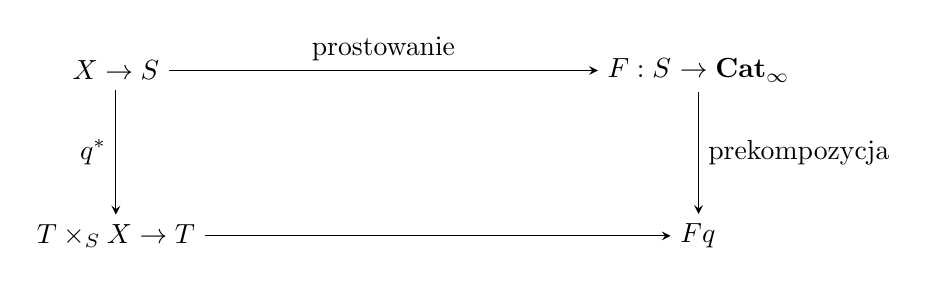
\begin{tikzpicture}[>=stealth]
 \node (X) at (0,2.1) {$X\to S$};
 \node (F) at (7.4,2.1) {$F:S^{\op}\to\mathbf{Cat}_{\infty}$};
 \node (Y) at (0,0) {$T\times_S X\to T$};
 \node (G) at (7.4,0) {$Fq^{\op}$};
 \draw[->] (X)--node[above] {prostowanie}(F);
 \draw[->] (Y)--(G);
 \draw[->] (X)--node[left] {$q^*$}(Y);
 \draw[->] (F)--node[right] {prekompozycja}(G);
\end{tikzpicture}
\end{center}
Diagram wyraża zgodność z morfizmem bazy $q:T\to S$ z dokładnością do równoważności, a nie równość konkretnych modeli zbiorów symplicjalnych.

\begin{przyklad}[Stały transport]\label{cat:ex:cartesian-constant-transport}
Dla quasi-kategorii $K$ rzut $S\times K\to S$ jest fibracją kartezjańską i kokartezjańską, odpowiadającą stałemu diagramowi o wartości $K$. Fibrację wewnętrzną otrzymujemy ze stwierdzenia~\ref{cat:ex:simplicial-product-fibration}. Dla $f:a\to b$ i $k\in K_0$ wybieramy krawędź $(f,s_0k)$. Jej kartezjańskość wynika z kryterium wypełniania rogów z ostatnią krawędzią będącą równoważnością w $K$ (twierdzenie o wypełnianiu rogów z równoważnościami z rozdziału~\ref{cat:sec:quasicategories}); składową w $S$ narzuca dolny sympleks. Kokartezjańskość otrzymujemy z kryterium dla pierwszej krawędzi. Włókna są izomorficzne z $K$, a transporty można wybrać jako identyczności. Dla kompleksu Kana $K$ rzut jest nawet fibracją Kana.
\end{przyklad}

Rozróżnienie fibracji kartezjańskich i kokartezjańskich odpowiada rozróżnieniu kontrawariantnych i kowariantnych diagramów. Prawa i lewa fibracja są szczególnymi przypadkami, w których wartości diagramu są typami homotopijnymi przestrzeni, a nie dowolnymi $\infty$-kategoriami.
